\documentclass[letterpaper,addpoints,answers]{exam}
\usepackage{graphicx}

\newcommand{\hide}[1]{%
}

\begin{document}

%\pagestyle{headandfoot}
%\lhead{
  %\large\bfseries Physics 107\\ 
  %Midterm Exam, June 15, 2009
%}
%\chead{}
%\rhead{
  %\large\bfseries Name:\enspace\makebox[2in]{\hrulefill}\\
  %\large\bfseries Signature:\enspace\makebox[2in]{\hrulefill}
%}
%\lfoot{}
%\cfoot[]{Page \thepage}
%\rfoot{}

\begin{coverpages}
 \large\bfseries
 
 \noindent 
 Physics 252: Electronics
 
 \vspace{2ex}
 \noindent
 Midterm Exam: February 28, 2013

 \vspace{5ex}
 \noindent 
 Name:\enspace\makebox[2in]{\hrulefill}\\

 \vspace{5ex}
 \noindent 
 This test is administered under the rules and regulations of the honor 
 code of the College of William \& Mary.  

 \vspace{5ex}
 \noindent 
 Show your work, and circle your answers.

 \vspace{5ex}
 \begin{center}
  \gradetable[v][questions]
 \end{center}
\end{coverpages}
 

\begin{questions}

\question

Consider the loaded voltage divider shown below.
\begin{center}
 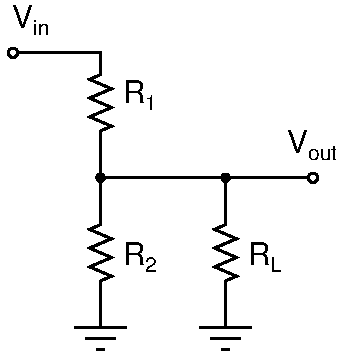
\includegraphics[width=0.25\textwidth]{./schematics/loaded_voltage_divider}
\end{center}
\begin{parts}
 \part[10]
  What must be the value of the load resistor $R_L$ to ensure maximum power transfer to
  it if $R_1 = 8\,\hbox{k}\Omega$ and $R_2 = 2\,\hbox{k}\Omega$?

  \vskip 3in
 \part[10]
  At the point of the maximum power transfer to the load resistor $R_L$, what
  is the value of the current passing through the resistor $R_1$
  if $V_{in} = 20\,\hbox{V}_{DC}$?

  \vskip 3in
\end{parts}


\pagebreak

\question

You are hired as a research assistant for an electronics lab. Your first
assignment is to characterize a black box (which seems to be a power
supply) given to you.

In a nearby lab book you find a series of measurements on this box.
In particular you find the voltage drop across several load resistors
connected to the box (see the table below).

\begin{center}
 \begin{tabular}{|c|c|}
  \hline
   $R_L$         &  $V_L$ \\ 
  \hline
   1\,k$\Omega$  &  20\,V \\
   50\,$\Omega$  &  5\,V  \\
  \hline
 \end{tabular}
\end{center}
 
\begin{parts}
 \part[10]
  Find the equivalent Th\'{e}venin voltage and resistance of this black box. 
  
  \vskip 3in
\end{parts}


\pagebreak

\question

For the circuits shown below specify if it is a low-pass, high-pass, band-pass or band-reject filter.

{\bf Hint:} It may be useful to think about the transfer function at high and low frequencies.
\begin{parts}
 \part[2] Circle one: band-pass \quad low-pass \quad high-pass \quad band-reject
 \begin{flushleft}
 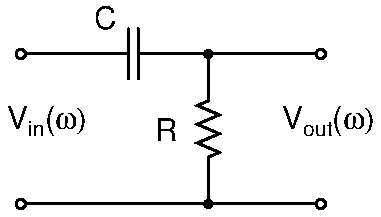
\includegraphics[height=0.7in]{./schematics/rc_high_pass}
 \end{flushleft}

 \part[2] Circle one: band-pass \quad low-pass \quad high-pass \quad band-reject
 \begin{flushleft}
 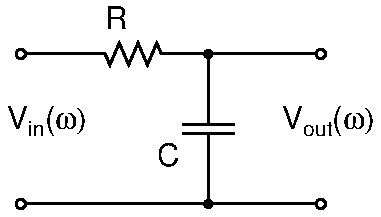
\includegraphics[height=0.7in]{./schematics/rc_low_pass}
 \end{flushleft}

 \part[2] Circle one: band-pass \quad low-pass \quad high-pass \quad band-reject
 \begin{flushleft}
 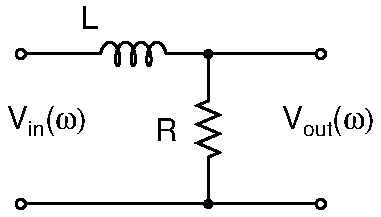
\includegraphics[height=0.7in]{./schematics/rl_low_pass}
 \end{flushleft}

 \part[2] Circle one: band-pass \quad low-pass \quad high-pass \quad band-reject
 \begin{flushleft}
 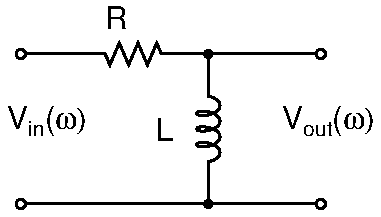
\includegraphics[height=0.7in]{./schematics/rl_high_pass}
 \end{flushleft}

 \part[4] Circle one: band-pass \quad low-pass \quad high-pass \quad band-reject
 \begin{flushleft}
 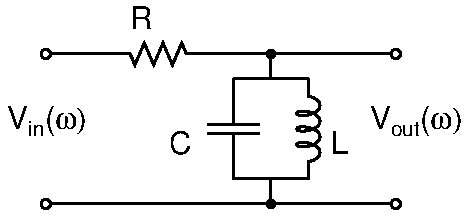
\includegraphics[height=0.7in]{./schematics/rlc_band_pass}
 \end{flushleft}

 \part[4] Circle one: band-pass \quad low-pass \quad high-pass \quad band-reject
 \begin{flushleft}
 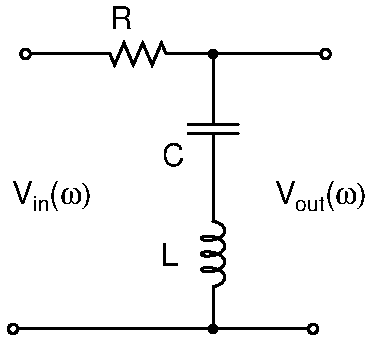
\includegraphics[height=1.1in]{./schematics/rlcnotch}
 \end{flushleft}

 \part[4] Circle one: band-pass \quad low-pass \quad high-pass \quad band-reject
 \begin{flushleft}
 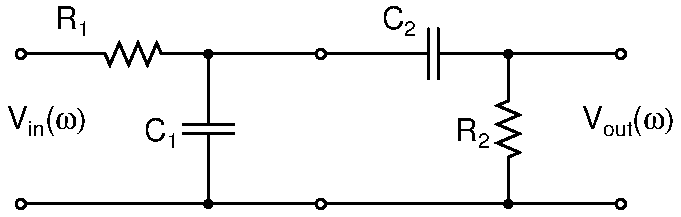
\includegraphics[height=0.7in]{./schematics/band_pass_filter}
 \end{flushleft}
\end{parts}

 
\pagebreak

\question

Consider the filter shown below.
\begin{center}
 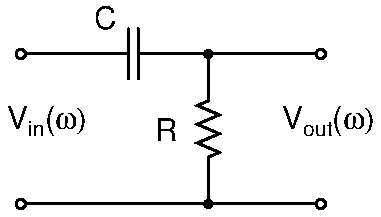
\includegraphics[width=0.25\textwidth]{./schematics/rc_high_pass}
\end{center}
\begin{parts}
 \part[5]
  What is the absolute value of the gain of this filter as a function of $\omega$?

  \vskip 1in
 \part[5]
  Sketch the Bode plot of the absolute value of the gain of this filter.

  \vskip 2in
 \part[10]
  Find the average power dissipated by the resistor if the amplitude of the input
  signal is $V_{in} = 1\,\hbox{V}$, $R = 500\,\Omega$,
  $C = 20\,\hbox{nF}$, and $\omega = \omega_{RC}$.
  
  \vskip 2in
 \part[10]
  At the same conditions as above, find the average power dissipated by the capacitor?

  \vskip 2in
\end{parts}


\pagebreak

\question

Your experimental apparatus generates useful signals at a frequency $f_s = 10$\,kHz 
with an amplitude $V_s = 0.01$\,V.  Unfortunately extremely strong noise couples
at a frequency $f_n = 0.1$\,kHz with an amplitude $V_n = 1$\,V.

During this problem you can use approximations and the simplified transfer
function representation.

\begin{parts}
 \part[5]
  What is the signal to noise ratio (SNR) coming from the apparatus?  Express your
  answer in either linear or dB scale, but be clear about which one you use.
  \vskip 1in
 \part[5]
  In a rush to improve the quality of the signal (i.e. SNR) you search
  through the lab and find a low-pass RC filter with $f_{3dB} = 1$\,kHz.

  What is the SNR at the output of this filter? Is it a good filter for the job?
  \vskip 2in
 \part[10]
  If it is up to you to design a filter, what kind of filter would you
  use?  Where would you place the $f_{3dB}$ of your filter for these
  noise conditions?  Draw a schematic of your filter.  What is the
  SNR after your improved filter?
  \vskip 3in
\end{parts}

\end{questions}

\end{document}
